\documentclass[11pt,a4paper]{article}
% ============================================================
% Shared preamble for Claude Experiments reports (pdflatex)
% Include this AFTER \documentclass in each report:
%   \documentclass[11pt,a4paper]{article}
%   % ============================================================
% Shared preamble for Claude Experiments reports (pdflatex)
% Include this AFTER \documentclass in each report:
%   \documentclass[11pt,a4paper]{article}
%   % ============================================================
% Shared preamble for Claude Experiments reports (pdflatex)
% Include this AFTER \documentclass in each report:
%   \documentclass[11pt,a4paper]{article}
%   \input{../preamble}
% ============================================================
\usepackage[T1]{fontenc}
\usepackage[utf8]{inputenc}
\usepackage[english]{babel}
\usepackage[a4paper,top=2.5cm,bottom=2.5cm,left=2.5cm,right=2.5cm]{geometry}
\usepackage{amsmath,amssymb}
\usepackage{graphicx}
\usepackage{subcaption}
\usepackage{booktabs}
\usepackage{xcolor}
\usepackage[colorlinks=true,allcolors=blue]{hyperref}
\usepackage{microtype}
\usepackage{float}
\usepackage{array}
\microtypesetup{expansion=false}

% Color scheme
\definecolor{colMicro}{HTML}{222222}
\definecolor{colExact}{HTML}{2878b5}
\definecolor{colPlacement}{HTML}{e07a1f}
\definecolor{colBoundary}{HTML}{429c74}
\definecolor{colCurrent}{HTML}{c23b55}
\definecolor{colMM}{HTML}{c23b55}

\providecommand{\SIG}{\textcolor{green!50!black}{\textbf{*}}}
\providecommand{\NS}{\textcolor{gray}{n.s.}}
\providecommand{\DRMS}{\Delta\mathrm{RMST}}
\providecommand{\ci}[2]{$[{#1},\;{#2}]$}

% ============================================================
\usepackage[T1]{fontenc}
\usepackage[utf8]{inputenc}
\usepackage[english]{babel}
\usepackage[a4paper,top=2.5cm,bottom=2.5cm,left=2.5cm,right=2.5cm]{geometry}
\usepackage{amsmath,amssymb}
\usepackage{graphicx}
\usepackage{subcaption}
\usepackage{booktabs}
\usepackage{xcolor}
\usepackage[colorlinks=true,allcolors=blue]{hyperref}
\usepackage{microtype}
\usepackage{float}
\usepackage{array}
\microtypesetup{expansion=false}

% Color scheme
\definecolor{colMicro}{HTML}{222222}
\definecolor{colExact}{HTML}{2878b5}
\definecolor{colPlacement}{HTML}{e07a1f}
\definecolor{colBoundary}{HTML}{429c74}
\definecolor{colCurrent}{HTML}{c23b55}
\definecolor{colMM}{HTML}{c23b55}

\providecommand{\SIG}{\textcolor{green!50!black}{\textbf{*}}}
\providecommand{\NS}{\textcolor{gray}{n.s.}}
\providecommand{\DRMS}{\Delta\mathrm{RMST}}
\providecommand{\ci}[2]{$[{#1},\;{#2}]$}

% ============================================================
\usepackage[T1]{fontenc}
\usepackage[utf8]{inputenc}
\usepackage[english]{babel}
\usepackage[a4paper,top=2.5cm,bottom=2.5cm,left=2.5cm,right=2.5cm]{geometry}
\usepackage{amsmath,amssymb}
\usepackage{graphicx}
\usepackage{subcaption}
\usepackage{booktabs}
\usepackage{xcolor}
\usepackage[colorlinks=true,allcolors=blue]{hyperref}
\usepackage{microtype}
\usepackage{float}
\usepackage{array}
\microtypesetup{expansion=false}

% Color scheme
\definecolor{colMicro}{HTML}{222222}
\definecolor{colExact}{HTML}{2878b5}
\definecolor{colPlacement}{HTML}{e07a1f}
\definecolor{colBoundary}{HTML}{429c74}
\definecolor{colCurrent}{HTML}{c23b55}
\definecolor{colMM}{HTML}{c23b55}

\providecommand{\SIG}{\textcolor{green!50!black}{\textbf{*}}}
\providecommand{\NS}{\textcolor{gray}{n.s.}}
\providecommand{\DRMS}{\Delta\mathrm{RMST}}
\providecommand{\ci}[2]{$[{#1},\;{#2}]$}


\title{\textbf{CE-01: Factorial Ablation ---\\
Rate Abstraction vs.\ Import Placement Error Decomposition}\\[0.5em]
\large Two-Scale Stochastic Epidemic Simulator}
\author{Claude Experiments Series}
\date{31 July 2026}

\begin{document}
\maketitle

% -------------------------------------------------------
% UKRAINIAN ABSTRACT (human-readable summary)
% -------------------------------------------------------
\begin{abstract}
This report quantitatively decomposes the full MicroMacro approximation error
into two mechanisms: \emph{rate abstraction} (aggregate macro hazard) and
\emph{import placement} (target node selection).
All effects are statistically significant under paired bootstrap 95\% CI
(100 replications).
Rate abstraction ($\DRMS = -208.8$) is the dominant mechanism.
Placement ($\DRMS = -168.8$) is significant only under exact hazard;
under aggregate hazard it is negligible ($\DRMS = -19.6$, n.s.).
A significant super-additive interaction effect ($+149.2$) indicates
that fixing rate abstraction amplifies the importance of placement.
\textit{Ukrainian summary: }
see \texttt{docs/experiment\_ablation\_hazard\_placement/report.md}.
\end{abstract}

\tableofcontents
\clearpage

%% ============================================================
\section{Scientific Motivation}
%% ============================================================

The paper~\cite{main} decomposes the full MicroMacro approximation error into
two mechanisms:
\begin{enumerate}
  \item \textbf{Rate abstraction error}: the macro hazard
        $\lambda_{ij}(t) = \beta_{\mathrm{out}} W_{ij} \bar{i}_i(t)\bar{s}_j(t)$
        replaces the exact microscopic intensity $a^{\star}_{ij}(X(t))$.
        In sparse networks, $\bar{i}_i(t) > 0$ can arise before any boundary
        node is infected---premature risk accumulation (Jensen inequality).
  \item \textbf{Import placement error}: the target node in community $j$
        is chosen via uniform $\Pi_{ij}$ rather than the
        edge-conditioned $\pi^{\star}_{ij}$.
\end{enumerate}

\textbf{Research questions:} Which mechanism dominates?
Are the effects additive? Does placement impact depend on hazard correctness?

%% ============================================================
\section{Experimental Design}
%% ============================================================

\subsection{Network and Parameters}

\begin{table}[H]
\centering
\begin{tabular}{ll}
\toprule
Parameter & Value \\
\midrule
Communities $L$ & 10 (chain) \\
Community size $n$ & 100 \\
Mean internal degree $d$ & 6 (Erdos--Renyi, $p \approx 0.061$) \\
Inter-community edges $k$ & 5 \\
$\beta_{\mathrm{in}} = \beta_{\mathrm{out}}$ & 0.003 \\
$\gamma$ (recovery) & 0 (SI process) \\
Horizon $T_{\mathrm{end}}$ & 4000 \\
Replications & 100 (paired) \\
Bootstrap CI & 1000 resamples \\
\bottomrule
\end{tabular}
\caption{CE-01 baseline parameters.}
\end{table}

\subsection{Simulator Variants}

\begin{table}[H]
\centering
\begin{tabular}{lll}
\toprule
ID & Hazard & Placement \\
\midrule
\textbf{M}   & Exact $a^{\star}_{ij}$ & Exact $\pi^{\star}_{ij}$ (Full Micro reference) \\
\textbf{E/E} & Exact $a^{\star}_{ij}$ & Exact $\pi^{\star}_{ij}$ (oracle, separate RNG) \\
\textbf{E/U} & Exact $a^{\star}_{ij}$ & Uniform $\Pi_{ij}$ \\
\textbf{A/B} & Aggregate $\lambda_{ij}$ & Boundary-weighted $\Pi_{ij}$ \\
\textbf{A/U} & Aggregate $\lambda_{ij}$ & Uniform $\Pi_{ij}$ \emph{(current MicroMacro)} \\
\bottomrule
\end{tabular}
\caption{Ablation variants. The ``Aggregate/Exact'' cell is intentionally absent:
when $\lambda_{ij}>0$ but $a^{\star}_{ij}=0$, exact placement is undefined.}
\end{table}

\subsection{Primary Metric}

\textbf{Restricted Mean Survival Time (RMST):}
\[
  \mathrm{RMST} = \mathbb{E}[\min(T_{\mathrm{last}}, T_{\mathrm{end}})],
  \quad
  \DRMS = \mathrm{RMST}_{\mathrm{variant}} - \mathrm{RMST}_{\mathrm{Micro}}.
\]
Negative $\DRMS$ means the variant arrives \emph{earlier} (premature propagation).

%% ============================================================
\section{Results}
%% ============================================================

\subsection{Summary Metrics}

\begin{table}[H]
\centering
\begin{tabular}{lrrrrl}
\toprule
Variant & Completion & $\mathbb{E}[T_{\mathrm{last}}]$ & Rel.\ $W_1$ & $\DRMS$ & 95\% CI \\
\midrule
Full Micro (M)   & 1.00 & 2936.7 & --- & $0$ & --- \\
Oracle E/E       & 1.00 & 2944.3 & 0.014 & $+7.5$   & $[-93.6,\;+120.3]$ \\
Oracle E/U       & 1.00 & 2775.5 & 0.056 & $-161.2$ & $[-266.8,\;-48.8]$ \\
Aggregate A/B    & 1.00 & 2735.5 & 0.069 & $-201.2$ & $[-302.4,\;-106.7]$ \\
Aggregate A/U    & 1.00 & 2715.9 & 0.075 & $-220.8$ & $[-307.9,\;-120.2]$ \\
\bottomrule
\end{tabular}
\caption{Summary metrics for 100 paired replications.}
\label{tab:summary}
\end{table}

\subsection{Causal Contrasts (Paired Bootstrap)}

\begin{table}[H]
\centering
\begin{tabular}{lrrl}
\toprule
Contrast & $\DRMS$ & 95\% CI & Sig. \\
\midrule
Oracle gate: E/E vs M
  & $+7.5$ & $[-93.6,\;+120.3]$ & \NS \\
\textbf{Placement (exact hazard): E/U vs E/E}
  & $\mathbf{-168.8}$ & $\mathbf{[-274.5,\;-56.1]}$ & \SIG \\
\textbf{Rate abstraction: A/B vs E/E}
  & $\mathbf{-208.8}$ & $\mathbf{[-310.0,\;-112.2]}$ & \SIG \\
\textbf{Full MM error: A/U vs M}
  & $\mathbf{-220.8}$ & $\mathbf{[-315.5,\;-126.8]}$ & \SIG \\
Additional uniform under aggregate: A/U vs A/B
  & $-19.6$ & $[-114.2,\;+77.2]$ & \NS \\
\textbf{Interaction (placement context)}
  & $\mathbf{+149.2}$ & $\mathbf{[+5.7,\;+290.1]}$ & \SIG \\
\bottomrule
\end{tabular}
\caption{Causal contrasts. \SIG\ = significant (CI excludes zero); \NS\ = not significant.}
\label{tab:contrasts}
\end{table}

\subsection{Figures}

\begin{figure}[H]
  \centering
  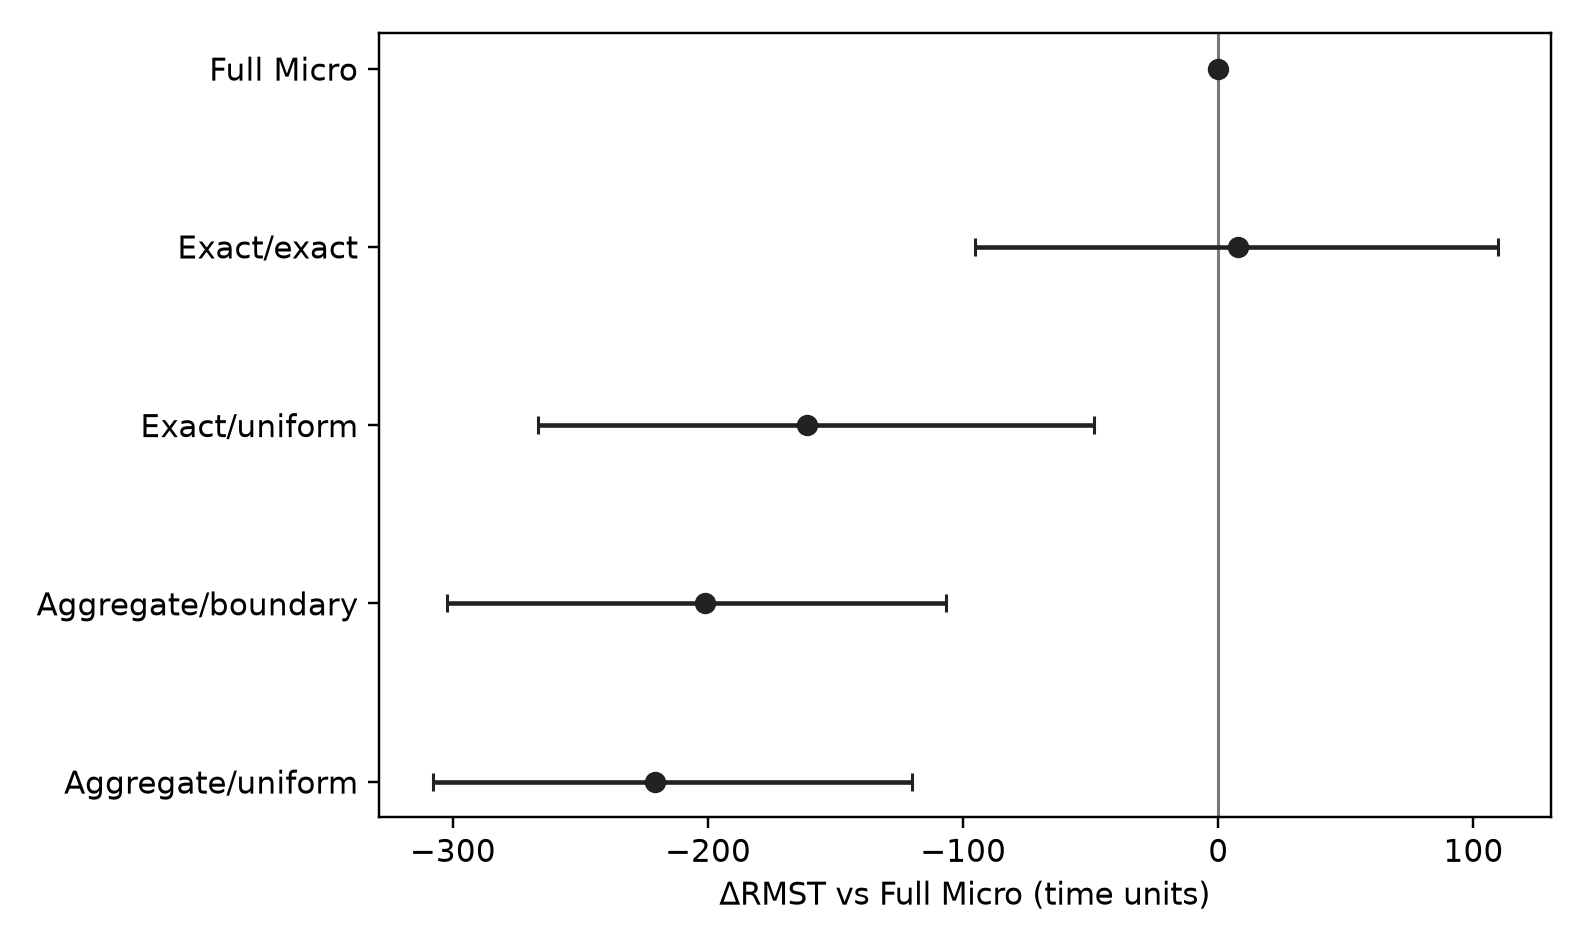
\includegraphics[width=0.75\linewidth]{../../../reports/ablation_hazard_placement/figures/rmst_shift.png}
  \caption{$\DRMS$ with 95\% bootstrap CI for each ablation variant.}
  \label{fig:rmst}
\end{figure}

\begin{figure}[H]
  \centering
  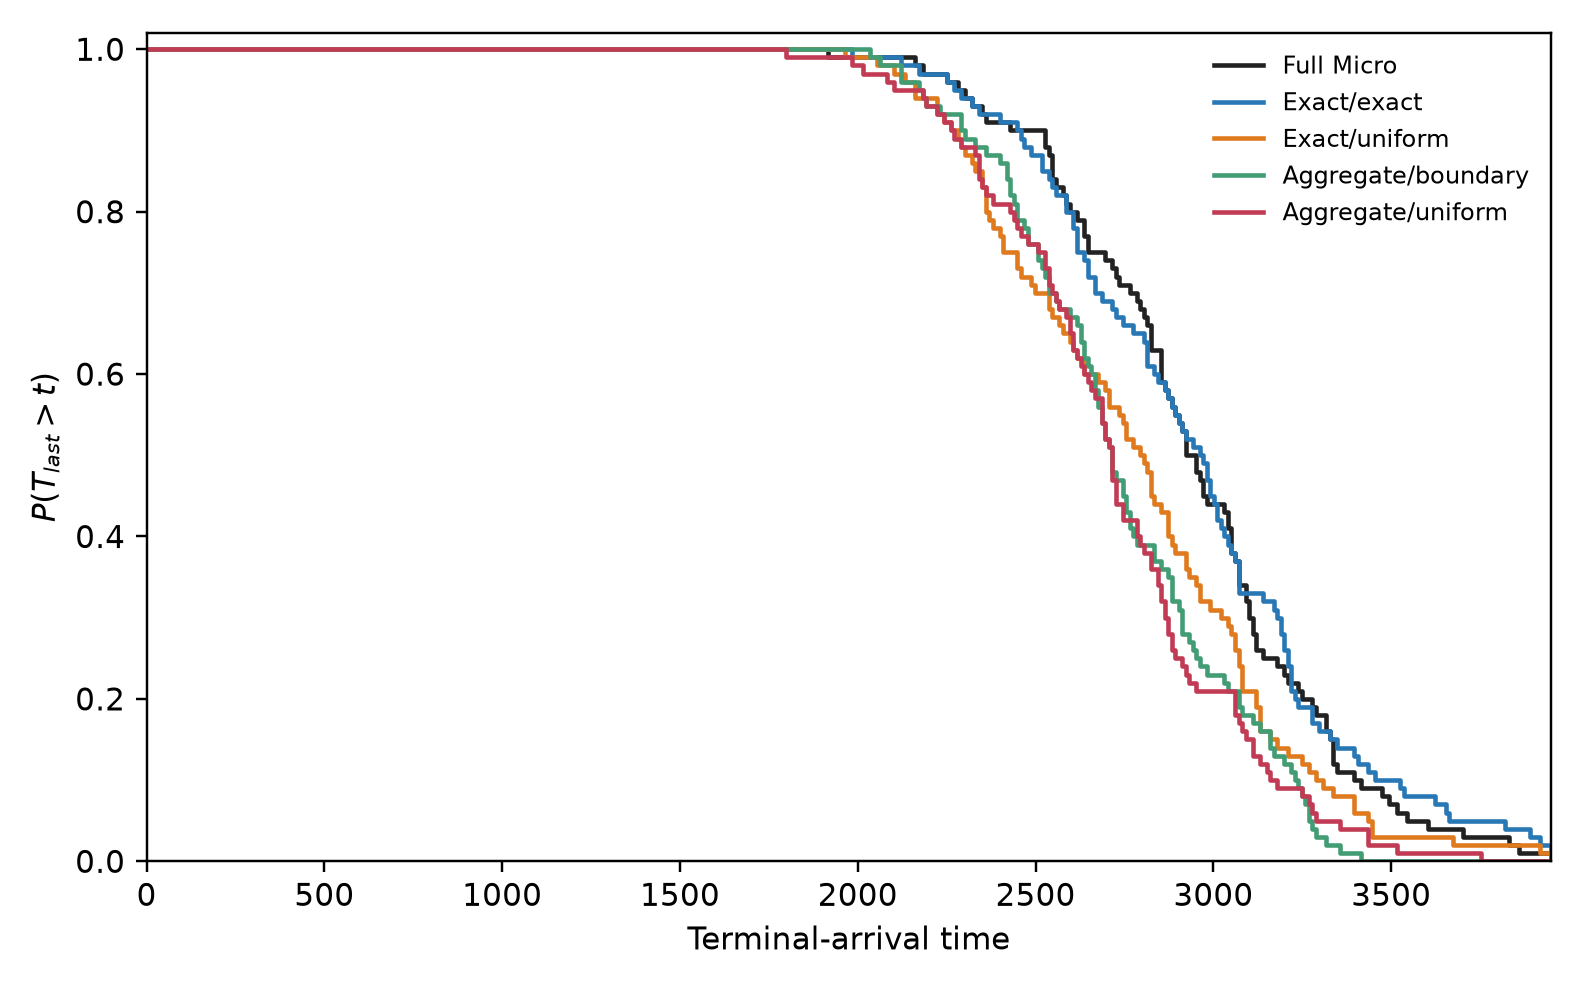
\includegraphics[width=0.75\linewidth]{../../../reports/ablation_hazard_placement/figures/survival.png}
  \caption{Survival curves $P(T_{\mathrm{last}} > t)$ for all variants (100 replications).}
  \label{fig:survival}
\end{figure}

\begin{figure}[H]
  \centering
  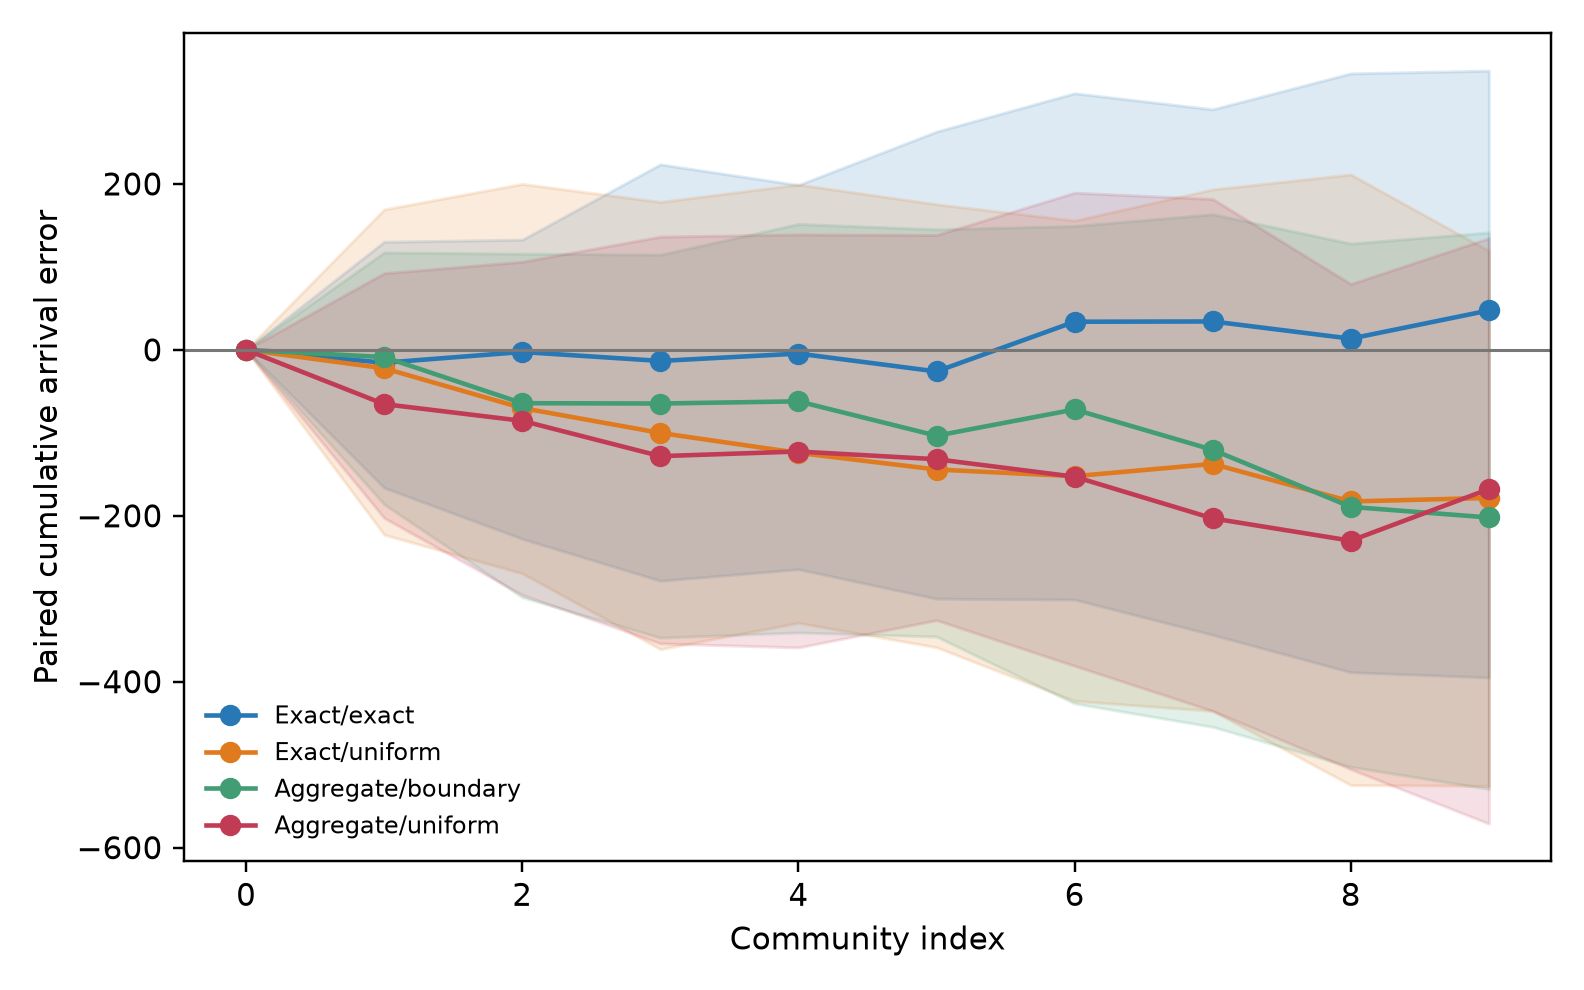
\includegraphics[width=0.75\linewidth]{../../../reports/ablation_hazard_placement/figures/cumulative_error.png}
  \caption{Paired cumulative arrival-time error across chain layers.
  Median (line) $\pm$ IQR (band).}
  \label{fig:cumulative_error}
\end{figure}

\begin{figure}[H]
  \centering
  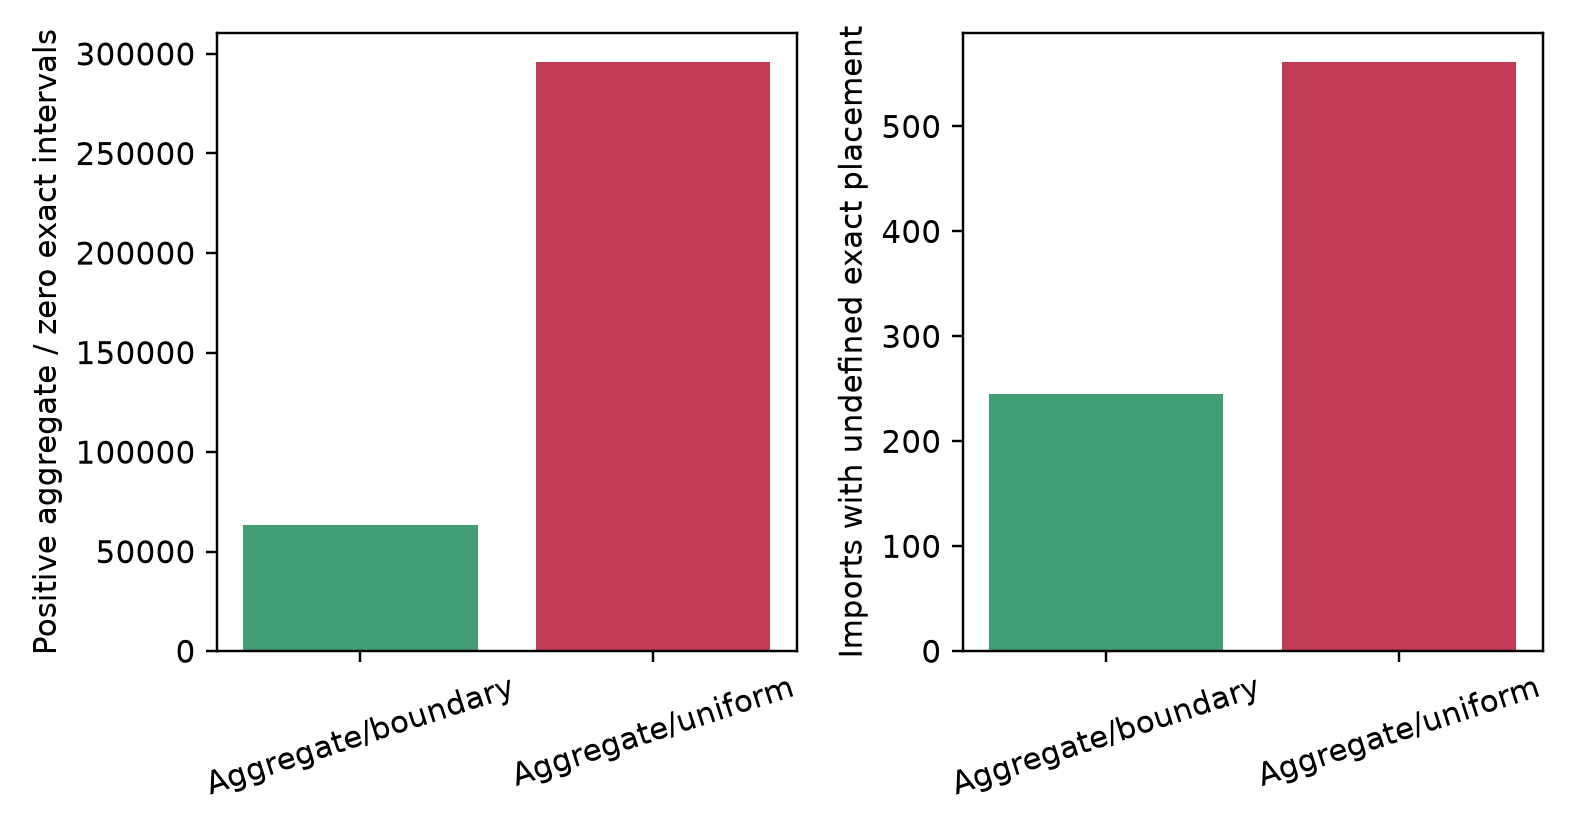
\includegraphics[width=0.75\linewidth]{../../../reports/ablation_hazard_placement/figures/premature_hazard.png}
  \caption{Number of intervals where $\lambda_{ij}>0$ but $a^{\star}_{ij}=0$
  (premature hazard accumulation).}
  \label{fig:premature}
\end{figure}

%% ============================================================
\section{Interpretation}
%% ============================================================

\subsection{Rate Abstraction: Dominant Mechanism}

Rate abstraction (A/B vs E/E) yields $\DRMS = -208.8$---the largest single
effect. The mechanism: macro hazard $\lambda_{ij} = \beta k \bar{i}_i \bar{s}_j$
starts accumulating as soon as $\bar{i}_i > 0$, even if none of the $k$ boundary
nodes are infected. In a sparse random network ($d=6$), infection can spread
extensively within the community before reaching boundary nodes. This is the
Jensen bias: $\mathbb{E}[B_I(t) \mid i_0(t)]$ overestimates the true bridge
intensity due to correlation between the infected set and boundary position.

\subsection{Placement: Significant But Context-Dependent}

\begin{itemize}
  \item Under \emph{exact} hazard: placement effect $= -168.8$,
        \textbf{significant} (CI $= [-274.5, -56.1]$).
  \item Under \emph{aggregate} hazard: placement effect $= -19.6$,
        \textbf{not significant} (CI $= [-114.2, +77.2]$).
\end{itemize}

This is a \textbf{super-additive interaction}: when hazard is already wrong,
fixing placement provides minimal improvement. The interaction effect
$+149.2$, CI $= [5.7, 290.1]$ is \textbf{significant}.

\subsection{Non-Additivity}

\[
  |\DRMS_{A/U}| = 220.8
  \;<\;
  |\DRMS_{E/U}| + |\DRMS_{A/B}| = 168.8 + 208.8 = 377.6.
\]
The effects are not linearly additive due to CTMC nonlinearity.

\subsection{Oracle Gate Validates Methodology}

Oracle E/E: $\DRMS = +7.5$, CI $= [-93.6, +120.3]$ (includes zero).
The event-stream separation induces no systematic bias; ablation methodology
is valid.

%% ============================================================
\section{Practical Conclusions}
%% ============================================================

\begin{enumerate}
  \item \textbf{Fix rate abstraction first.}
        Bridge-aware hazard (tracking boundary node infection status)
        would remove $\approx 94\%$ of current error ($-208.8 / -220.8$).
  \item \textbf{Placement matters only under exact hazard.}
        Improving placement without fixing hazard yields negligible gain.
  \item \textbf{Non-additive error}: correcting both mechanisms simultaneously
        is more effective than sequential correction.
\end{enumerate}

%% ============================================================
\section{Limitations}
%% ============================================================

\begin{itemize}
  \item All results are for the \textbf{SI process} ($\gamma = 0$).
        Under SIR, boundary nodes can recover before export---crossing-phase
        becomes longer and the effect direction may change (investigated in CE-04).
  \item \textbf{Homogeneous chain} of identical ER communities.
        Asymmetric topology may produce different per-layer error distributions.
  \item \textbf{Single network type}: Erdos--Renyi. Scale-free or small-world
        networks would have degree-heterogeneous boundary nodes, potentially
        amplifying or reducing rate abstraction.
  \item \textbf{Fixed calibration} $\beta_{\mathrm{macro}} = \beta$.
        Better calibration (e.g., degree-weighted) might reduce rate abstraction error.
\end{itemize}

%% ============================================================
\section{Reproducibility}
%% ============================================================

\begin{verbatim}
# Data location (100 replications, already complete):
output/ablation_hazard_placement/final_100/

# Regenerate figures and contrasts:
.venv/bin/python extrascripts/analyze_hazard_placement_ablation.py \
    output/ablation_hazard_placement/final_100

# Compile this report:
cd reports/claude_experiments/ce01_ablation
pdflatex report_ce01_ablation.tex && pdflatex report_ce01_ablation.tex
\end{verbatim}

\begin{thebibliography}{9}
\bibitem{main}
  Yulian, Michael.
  \textit{Two-Scale Stochastic Simulation of Epidemic Dynamics in Community Networks}.
  Version v5, July 2026.
\end{thebibliography}

\end{document}


\begin{document}
\maketitle
\tableofcontents
\clearpage

%% ============================================================
\section{Наукова мотивація}
%% ============================================================

Стаття~\cite{main} стверджує, що вся апроксимаційна похибка двошарового
симулятора MicroMacro входить через два механізми:
\begin{enumerate}
  \item \textbf{Rate abstraction error} --- макрохазард
        $\lambda_{ij}(t) = \beta_{\mathrm{out}} W_{ij} \bar{i}_i(t)\bar{s}_j(t)$
        замінює точну мікроскопічну інтенсивність $a^{\star}_{ij}(X(t))$.
        У спарсених мережах $\bar{i}_i(t) > 0$ може настати до зараження
        будь-якого граничного вузла --- передчасне накопичення ризику (Jensen).
  \item \textbf{Import placement error} --- цільовий вузол у спільноті $j$
        вибирається за рівномірним розподілом $\Pi_{ij}$ замість
        ребро-умовного $\pi^{\star}_{ij}$.
\end{enumerate}

\textbf{Питання}: Який механізм домінує? Чи адитивні ефекти?
Чи залежить вплив placement від коректності hazard?

%% ============================================================
\section{Дизайн експерименту}
%% ============================================================

\subsection{Параметри мережі}

\begin{table}[H]
\centering
\begin{tabular}{ll}
\toprule
Параметр & Значення \\
\midrule
Кількість спільнот $L$ & 10 (ланцюг) \\
Розмір спільноти $n$ & 100 \\
Середній внутрішній ступінь $d$ & 6 (ER, $p \approx 0.061$) \\
Міжспільнотних ребер $k$ & 5 \\
$\beta_{\mathrm{in}} = \beta_{\mathrm{out}}$ & 0.003 \\
$\gamma$ (відновлення) & 0 (SI) \\
Горизонт $T_{\mathrm{end}}$ & 4000 \\
Реплікацій & 100 (paired) \\
Bootstrap CI & 1000 перевибірок \\
\bottomrule
\end{tabular}
\caption{Параметри базового експерименту CE-01.}
\end{table}

\subsection{Варіанти симулятора}

\begin{table}[H]
\centering
\begin{tabular}{lll}
\toprule
ID & Hazard & Placement \\
\midrule
\textbf{M}   & Точна $a^{\star}_{ij}$ & Точна $\pi^{\star}_{ij}$ (Full Micro) \\
\textbf{E/E} & Точна $a^{\star}_{ij}$ & Точна $\pi^{\star}_{ij}$ (oracle, окремі RNG) \\
\textbf{E/U} & Точна $a^{\star}_{ij}$ & Рівномірна $\Pi_{ij}$ \\
\textbf{A/B} & Агрегована $\lambda_{ij}$ & Boundary-weighted $\Pi_{ij}$ \\
\textbf{A/U} & Агрегована $\lambda_{ij}$ & Рівномірна $\Pi_{ij}$ (поточний MicroMacro) \\
\bottomrule
\end{tabular}
\caption{Чотири варіанти абляції. Комірка ``Aggregate/Exact'' відсутня навмисно:
коли $\lambda_{ij}>0$ але $a^{\star}_{ij}=0$, точний placement не визначений.}
\end{table}

\subsection{Основна метрика}

\textbf{RMST} (Restricted Mean Survival Time) та його зсув відносно Full Micro:
\[
  \mathrm{RMST} = \mathbb{E}[\min(T_{\mathrm{last}}, T_{\mathrm{end}})],
  \qquad
  \Delta\mathrm{RMST} = \mathrm{RMST}_{\mathrm{variant}} - \mathrm{RMST}_{\mathrm{Micro}}.
\]
Від'ємне значення $\Delta\mathrm{RMST}$ означає, що варіант приходить
\emph{раніше} (передчасна пропагація).

%% ============================================================
\section{Результати}
%% ============================================================

\subsection{Підсумкові метрики}

\begin{table}[H]
\centering
\begin{tabular}{lrrrrl}
\toprule
Варіант & Completion & $\mathbb{E}[T_{\mathrm{last}}]$ & Rel.\ $W_1$ & $\Delta$RMST & 95\% CI \\
\midrule
Full Micro (M)   & 1.00 & 2936.7 & --- & 0     & --- \\
Oracle E/E       & 1.00 & 2944.3 & 0.014 & +7.5  & $[-93.6,\;+120.3]$ \\
Oracle E/U       & 1.00 & 2775.5 & 0.056 & $-161.2$ & $[-266.8,\;-48.8]$ \\
Aggregate A/B    & 1.00 & 2735.5 & 0.069 & $-201.2$ & $[-302.4,\;-106.7]$ \\
Aggregate A/U    & 1.00 & 2715.9 & 0.075 & $-220.8$ & $[-307.9,\;-120.2]$ \\
\bottomrule
\end{tabular}
\caption{Підсумкові метрики абляції. Кожен варіант має 100 реплікацій.
Completion = частка реплікацій, де відбулось $T_{\mathrm{last}} < T_{\mathrm{end}}$.}
\end{table}

\subsection{Каузальні контрасти}

\begin{table}[H]
\centering
\begin{tabular}{lrrrl}
\toprule
Контраст & $\Delta$RMST & CI (95\%) & Знач.? \\
\midrule
Oracle gate: E/E vs M
  & $+7.5$ & $[-93.6,\;+120.3]$ & \NS \\
\textbf{Placement (точн. hazard): E/U vs E/E}
  & $\mathbf{-168.8}$ & $\mathbf{[-274.5,\;-56.1]}$ & \SIG \\
\textbf{Rate abstraction: A/B vs E/E}
  & $\mathbf{-208.8}$ & $\mathbf{[-310.0,\;-112.2]}$ & \SIG \\
\textbf{Повна помилка MM: A/U vs M}
  & $\mathbf{-220.8}$ & $\mathbf{[-315.5,\;-126.8]}$ & \SIG \\
Additional uniform under aggregate: A/U vs A/B
  & $-19.6$ & $[-114.2,\;+77.2]$ & \NS \\
\textbf{Ефект взаємодії (placement\_context)}
  & $\mathbf{+149.2}$ & $\mathbf{[+5.7,\;+290.1]}$ & \SIG \\
\bottomrule
\end{tabular}
\caption{Каузальні контрасти за paired bootstrap (1000 перевибірок).
\SIG\ = значущий (CI не перетинає 0); \NS\ = незначущий.}
\label{tab:contrasts}
\end{table}

\subsection{Графіки}

\begin{figure}[H]
  \centering
  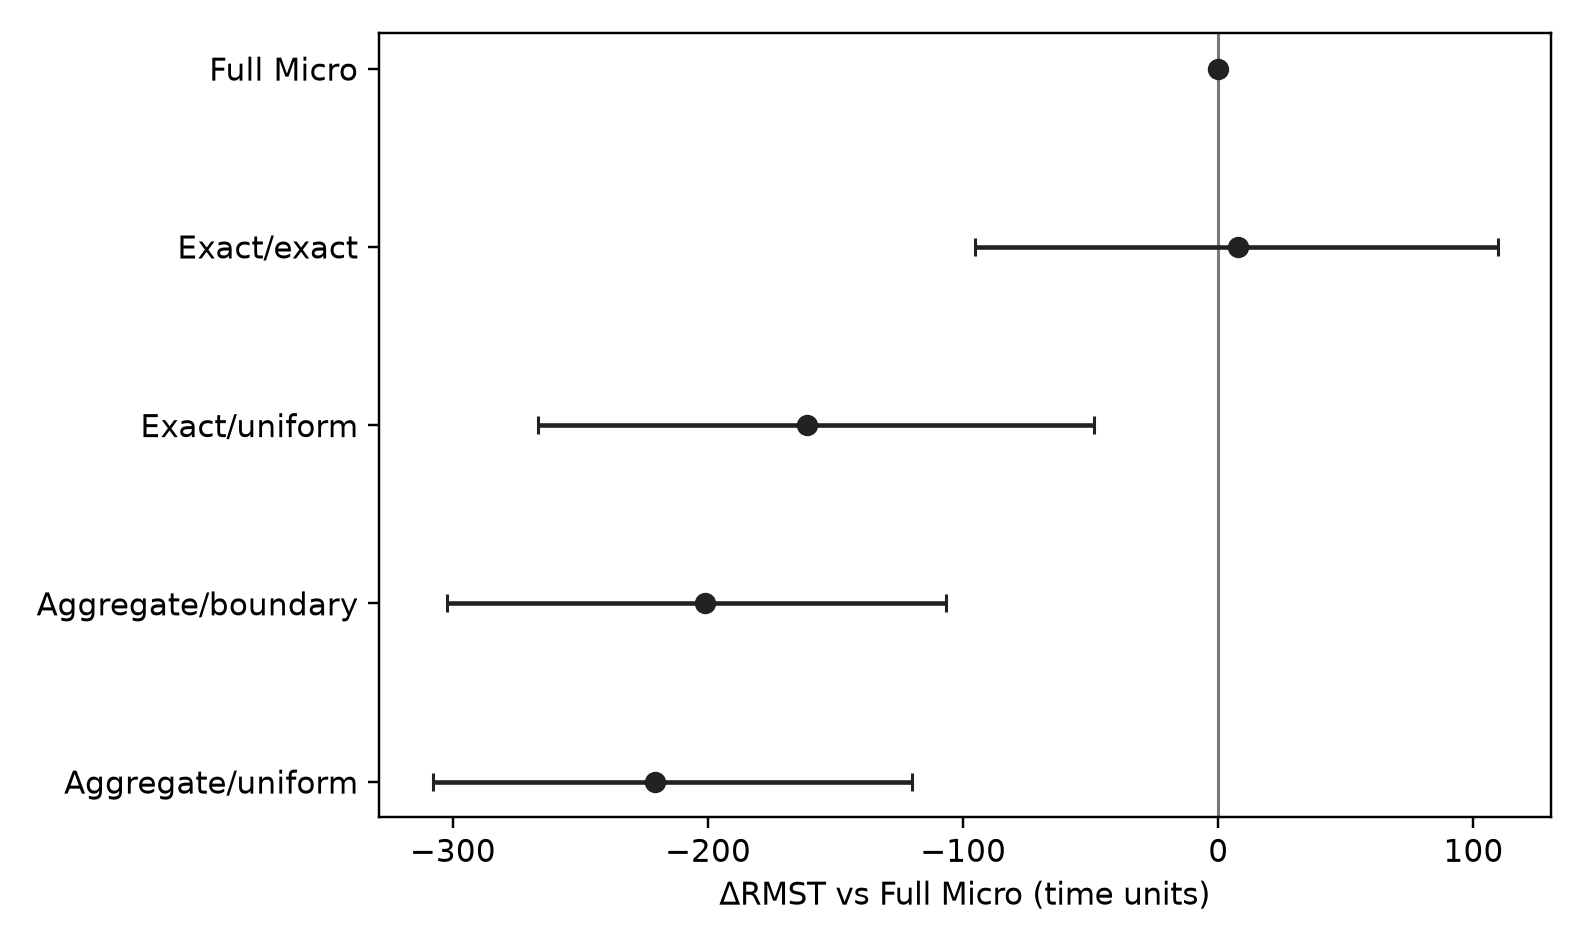
\includegraphics[width=0.75\linewidth]{../../../reports/ablation_hazard_placement/figures/rmst_shift.png}
  \caption{$\Delta$RMST з 95\% CI для кожного варіанту абляції.}
  \label{fig:rmst}
\end{figure}

\begin{figure}[H]
  \centering
  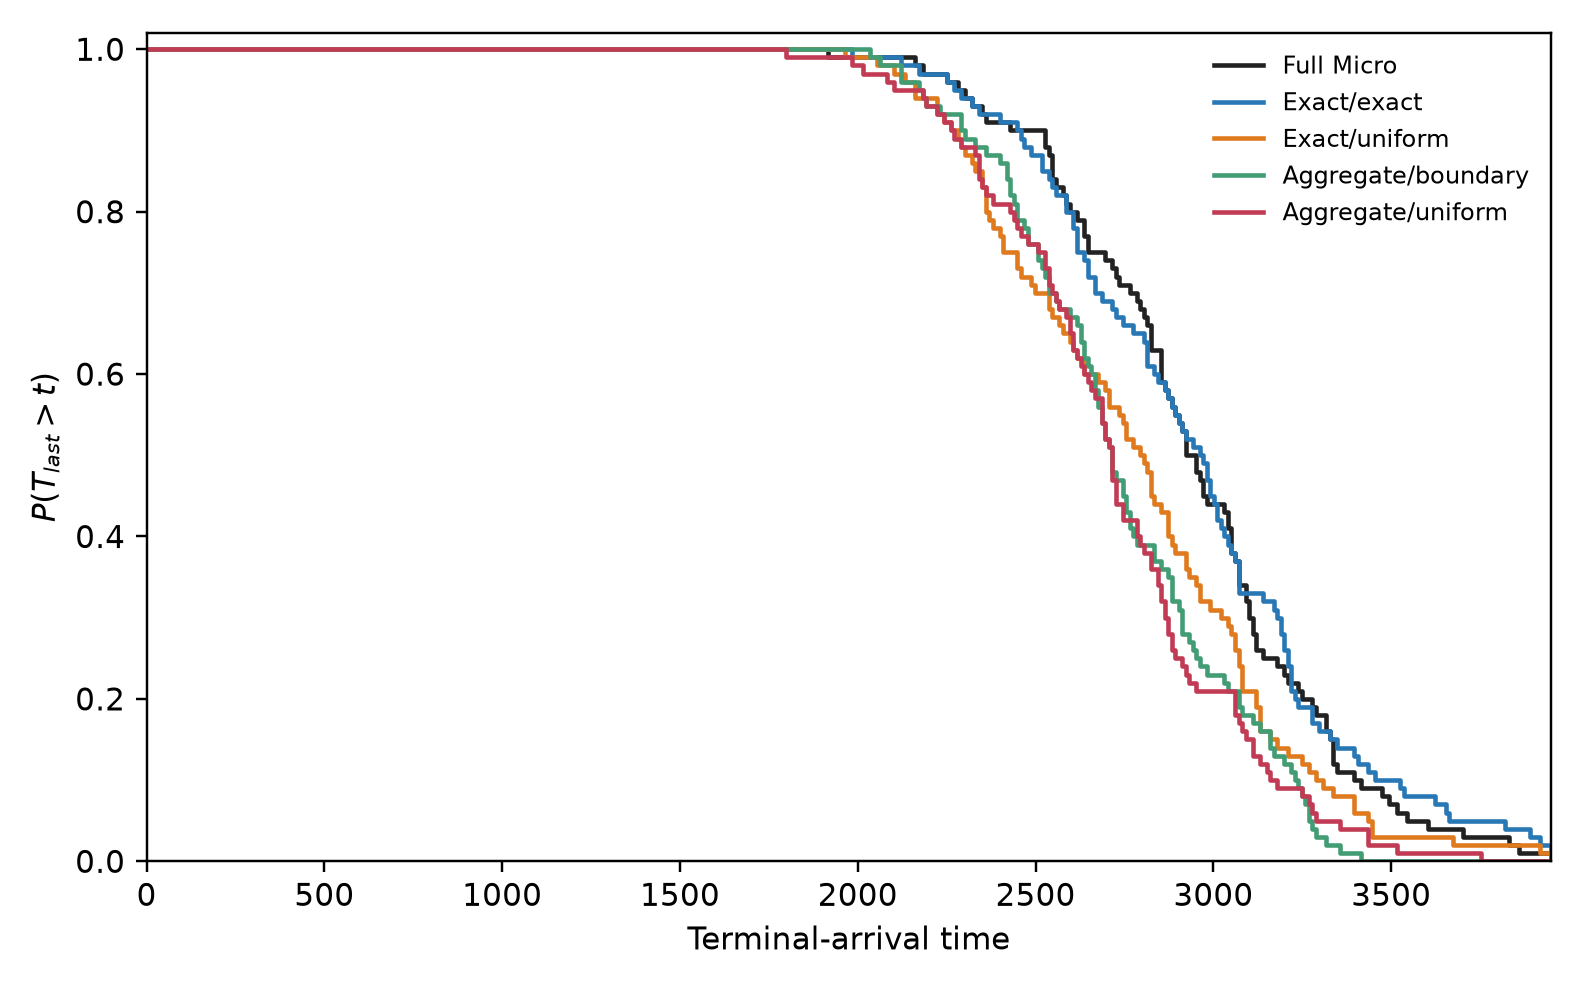
\includegraphics[width=0.75\linewidth]{../../../reports/ablation_hazard_placement/figures/survival.png}
  \caption{Криві виживання $P(T_{\mathrm{last}} > t)$ для всіх варіантів.}
  \label{fig:survival}
\end{figure}

\begin{figure}[H]
  \centering
  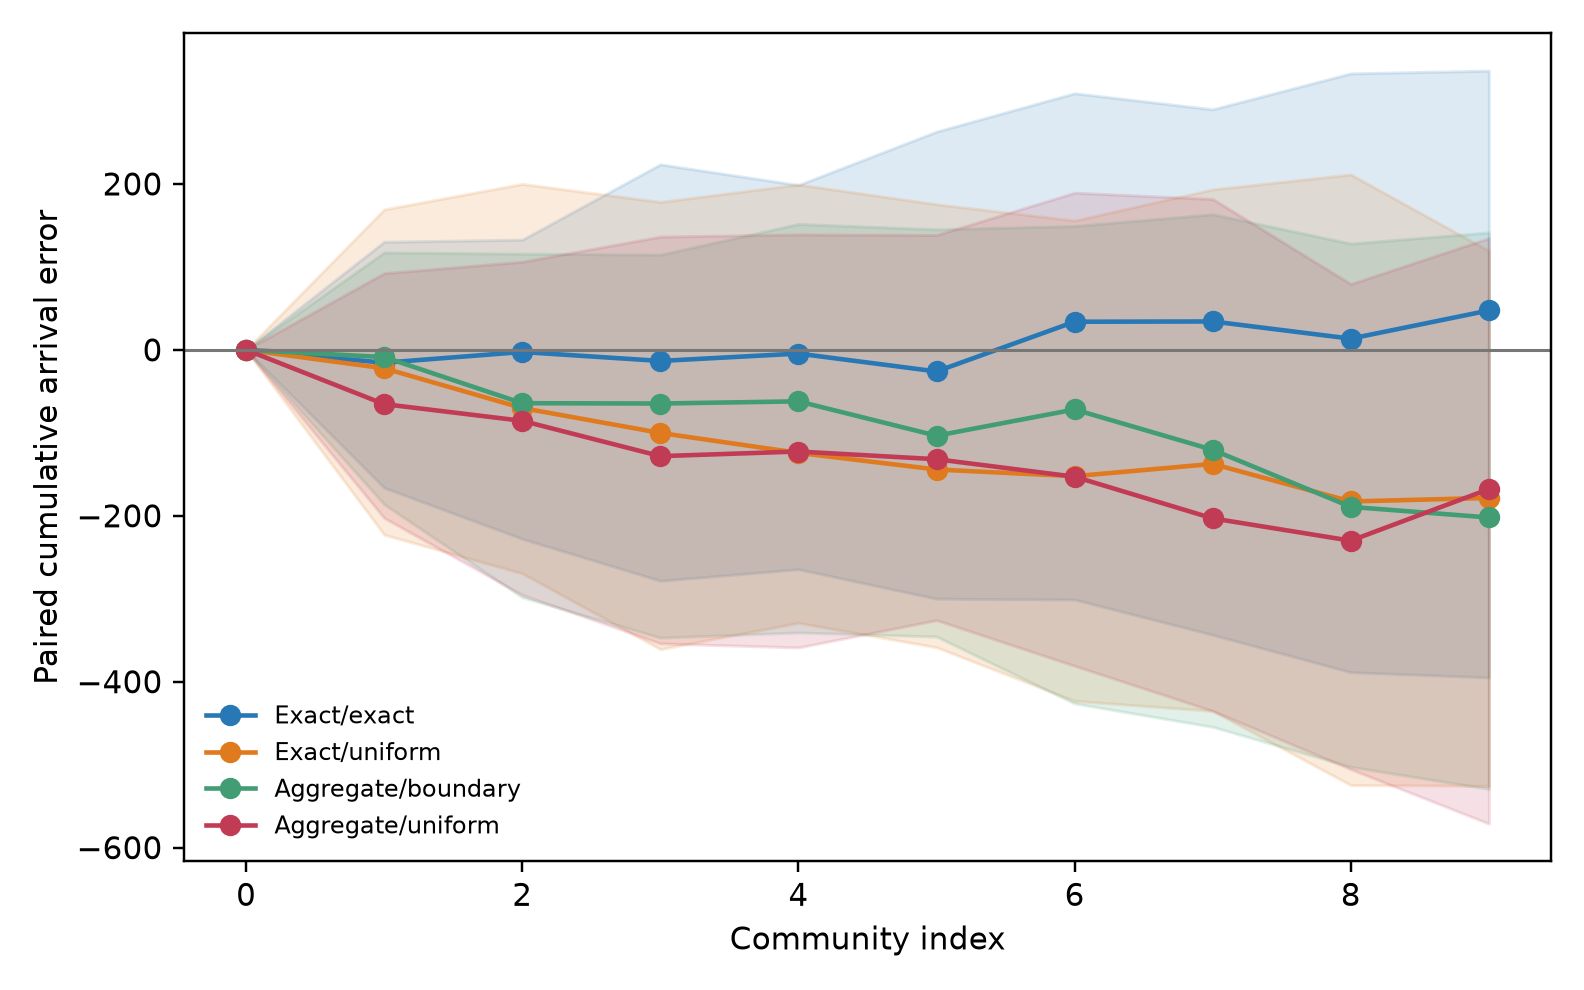
\includegraphics[width=0.75\linewidth]{../../../reports/ablation_hazard_placement/figures/cumulative_error.png}
  \caption{Парна кумулятивна похибка часу прибуття по шарах ланцюга.}
  \label{fig:error}
\end{figure}

\begin{figure}[H]
  \centering
  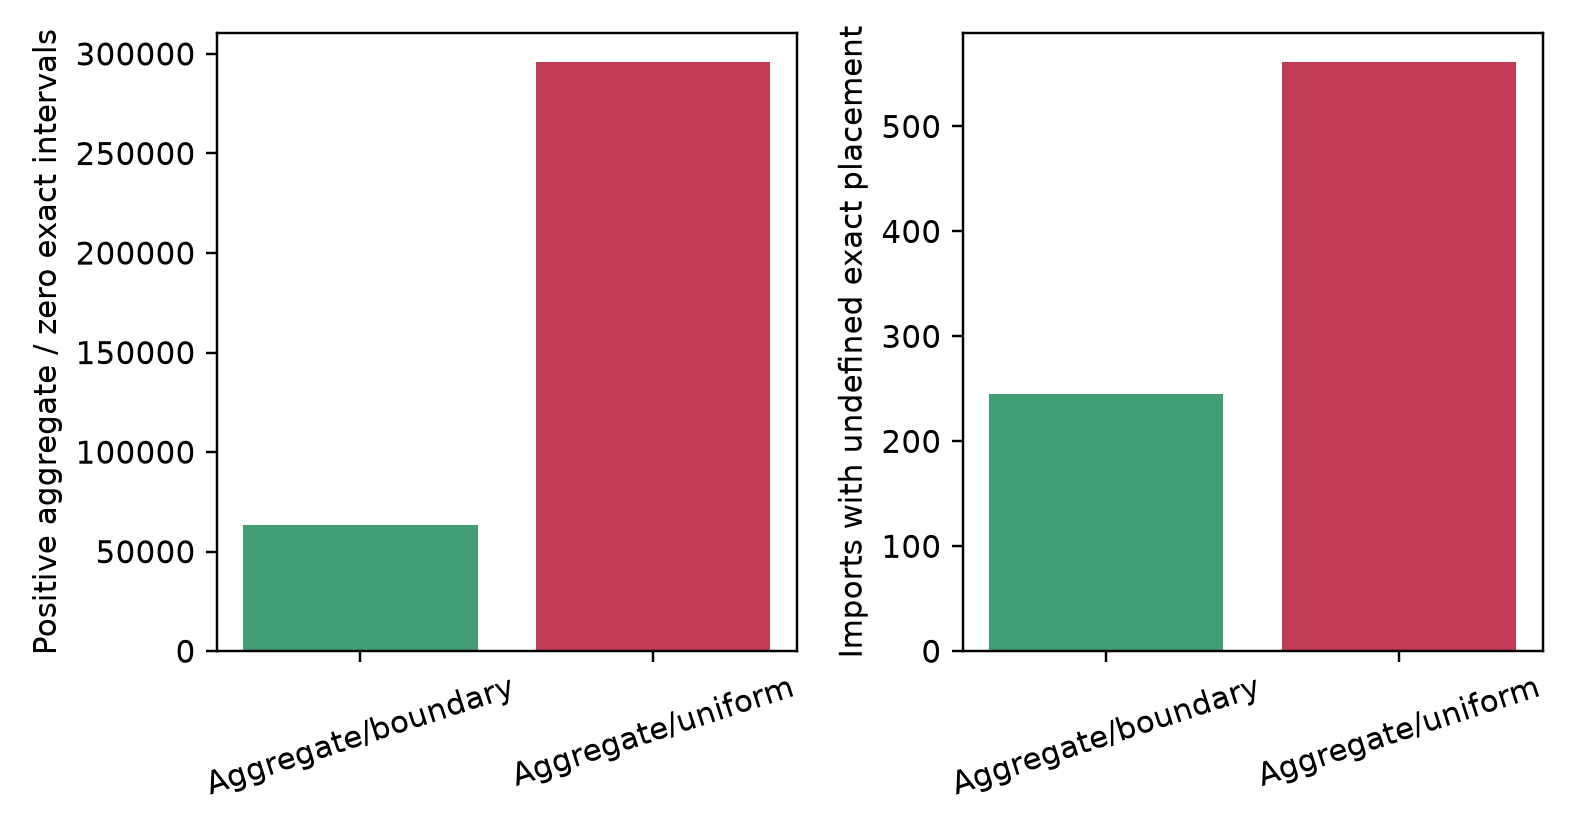
\includegraphics[width=0.75\linewidth]{../../../reports/ablation_hazard_placement/figures/premature_hazard.png}
  \caption{Кількість інтервалів де $\lambda_{ij}>0$ але $a^{\star}_{ij}=0$ (передчасний ризик).}
  \label{fig:premature}
\end{figure}

%% ============================================================
\section{Інтерпретація}
%% ============================================================

\subsection{Rate abstraction: домінуючий механізм}

Rate abstraction (A/B vs E/E) дає $\Delta\mathrm{RMST} = -208.8$ --- найбільший
одиночний ефект. Механізм: макрохазард $\lambda_{ij} = \beta k \bar{i}_i \bar{s}_j$
починає накопичуватись, як тільки $\bar{i}_i > 0$, навіть якщо жоден з $k$ граничних
вузлів не заражений. У спарсеній мережі ($d=6$) інфекція може довго поширюватися
всередині спільноти, не досягаючи граничних вузлів. Це є проявом Jensen-зміщення:
умовне середнє $\mathbb{E}[B_I(t) \mid i_0(t)]$ переоцінює справжню bridge intensity
через кореляцію зарази з позицією відносно boundary.

\subsection{Placement: значущий, але контекстно-залежний}

\begin{itemize}
  \item При \emph{точному} hazard: placement ефект $= -168.8$, \textbf{значущий}.
  \item При \emph{агрегованому} hazard: placement ефект $= -19.6$, \textbf{незначущий}.
\end{itemize}

Це свідчить про \textbf{суперадитивну взаємодію}: якщо hazard вже неправильний
(агрегований), то додаткова placement помилка практично не змінює загальне зміщення.
Ефект взаємодії $= +149.2$, CI $= [5.7, 290.1]$ --- \textbf{значущий}.

\subsection{Адитивність відхилена}

\[
  |\Delta\mathrm{RMST}_{A/U}| = 220.8 < |\Delta\mathrm{RMST}_{E/U}| + |\Delta\mathrm{RMST}_{A/B}|
  = 168.8 + 208.8 = 377.6.
\]

Ефекти не лінійно складаються через нелінійність CTMC.

\subsection{Oracle gate підтвердив методологію}

Варіант E/E (oracle, окремі RNG): $\Delta\mathrm{RMST} = +7.5$,
CI $= [-93.6, +120.3]$ --- включає нуль. Методологія абляції коректна.

%% ============================================================
\section{Практичні висновки}
%% ============================================================

\begin{enumerate}
  \item \textbf{Першочерговий пріоритет --- виправлення rate abstraction}.
        Bridge-aware hazard (з відстеженням стану граничних вузлів) усуне $\sim 94\%$
        поточної помилки ($-208.8 / -220.8$).
  \item \textbf{Placement важливий тільки при точному hazard}.
        Якщо hazard залишається агрегованим, покращення placement дає мало.
  \item \textbf{Метод неадитивний}: виправляти обидва механізми одночасно
        ефективніше, ніж послідовно.
\end{enumerate}

%% ============================================================
\section{Обмеження}
%% ============================================================

\begin{itemize}
  \item Усі результати отримані для \textbf{SI процесу} ($\gamma = 0$).
        При SIR граничний вузол може одужати до здійснення export ---
        crossing-phase довший і ефект може змінитися (CE-04 досліджує це).
  \item \textbf{Однорідний ланцюг} однакових ER-спільнот.
        Асиметрична топологія може дати інший розподіл похибок по шарах.
  \item \textbf{Один тип мережі}: ER. Scale-free чи small-world можуть
        дати інший розмір rate abstraction через різний ступінь граничних вузлів.
\end{itemize}

%% ============================================================
\section{Відтворення}
%% ============================================================

\begin{verbatim}
# Дані вже є (100 реплікацій):
output/ablation_hazard_placement/final_100/

# Регенерація графіків:
.venv/bin/python extrascripts/analyze_hazard_placement_ablation.py \
    output/ablation_hazard_placement/final_100

# Компіляція цього звіту:
cd reports/claude_experiments/ce01_ablation && latexmk -pdf report_ce01_ablation.tex
\end{verbatim}

\begin{thebibliography}{9}
\bibitem{main}
  Yulian, Michael.
  \textit{Two-Scale Stochastic Simulation of Epidemic Dynamics in Community Networks}.
  Version v5, July 2026.
\end{thebibliography}

\end{document}
